\documentclass{beamer}
\usepackage[utf8]{inputenc}
\usetheme[pageofpages=of,bullet=square,
	titleline=true,
	alternativetitlepage=true,
	titlepagelogo=images/xkcd-correlation2.jpg]{Torino}

\author{Statistical Reasoning\\and Quantitative Methods}
\title{Introduction}
\institute{François Briatte \& Ivaylo Petev}
\date{Session 1}

\include{settings}

\begin{document}
		
	\begin{frame}[t,plain]
		\titlepage
	\end{frame}
	
	\begin{frame}[t]{Outline}
		\tableofcontents[hideallsubsections]
	\end{frame}
	
	\section{Introduction}
	
	\subsection{Reality}
	
	\subsubsection{… predictable}
	
	\begin{frame}[t]{Reality is \red{predictable}}
		\href{http://articles.latimes.com/2010/aug/21/local/la-me-predictcrime-20100427-1}{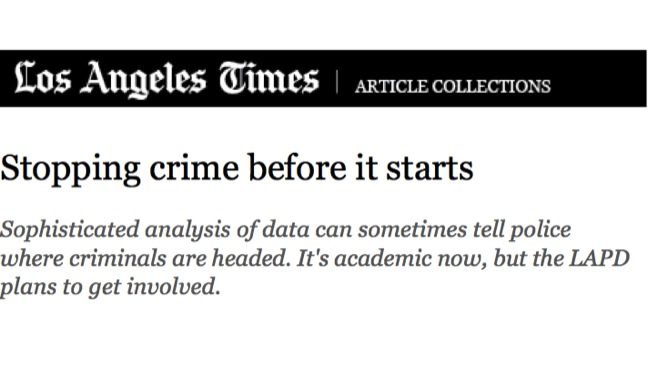
\includegraphics[width=\textwidth]{images/predicting.jpg}}
	\end{frame}
	
	\subsubsection{… visualizable}
	
	\begin{frame}[t]{Reality is \red{visualizable}}
		\href{http://www.bricoleurbanism.org/whimsicality/urban-fabric-form-comparison/}{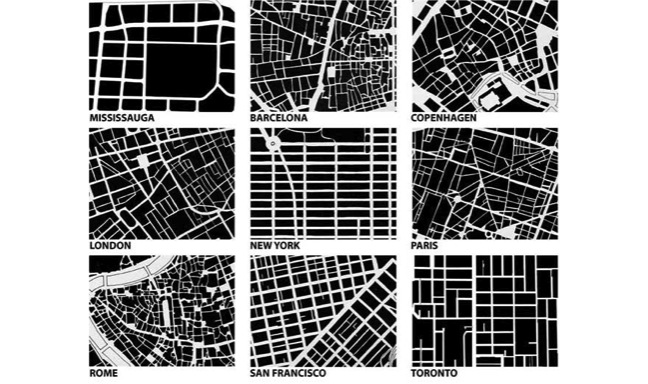
\includegraphics[width=\textwidth]{images/visualize.jpg}}
	\end{frame}

	\subsubsection{… multidimensional}
	
	\begin{frame}[t]{Reality is \red{multidimensional}}
		\href{http://www.last.fm/user/phnk1/library}{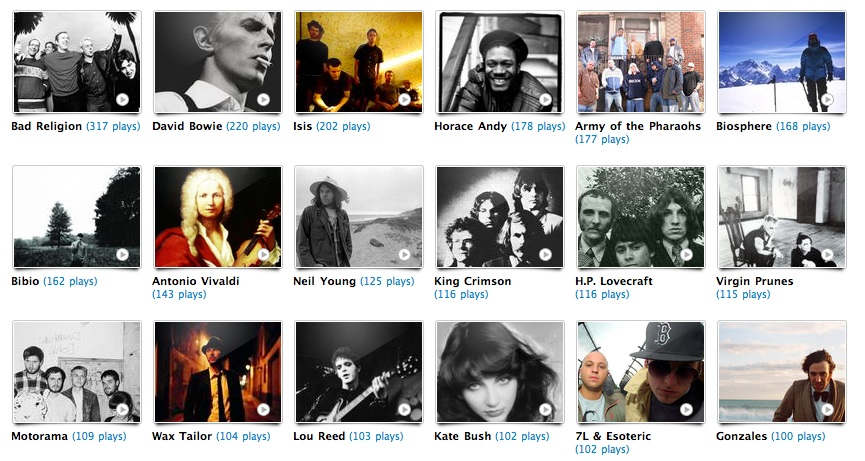
\includegraphics[width=\textwidth]{images/lastfm.jpg}}
	\end{frame}

	\begin{frame}[c]{Reality is \red{relational}}

		\begin{columns}[T]
			\column{.45\textwidth}
			\begin{center}
				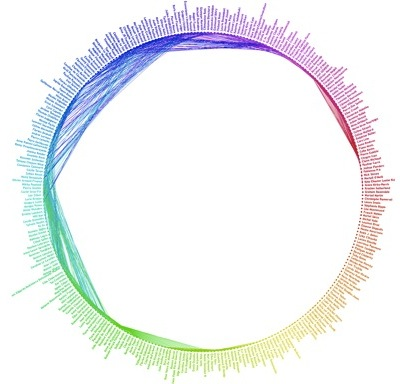
\includegraphics[height=4cm]{images/friendwheel.jpg}\\
				\vspace{0.74cm}
				Friendship ties on Facebook
			\end{center}
			\column{.45\textwidth}
			\begin{center}
				\href{http://www.sociology.columbia.edu/pdf-files/bearmanarticle.pdf}{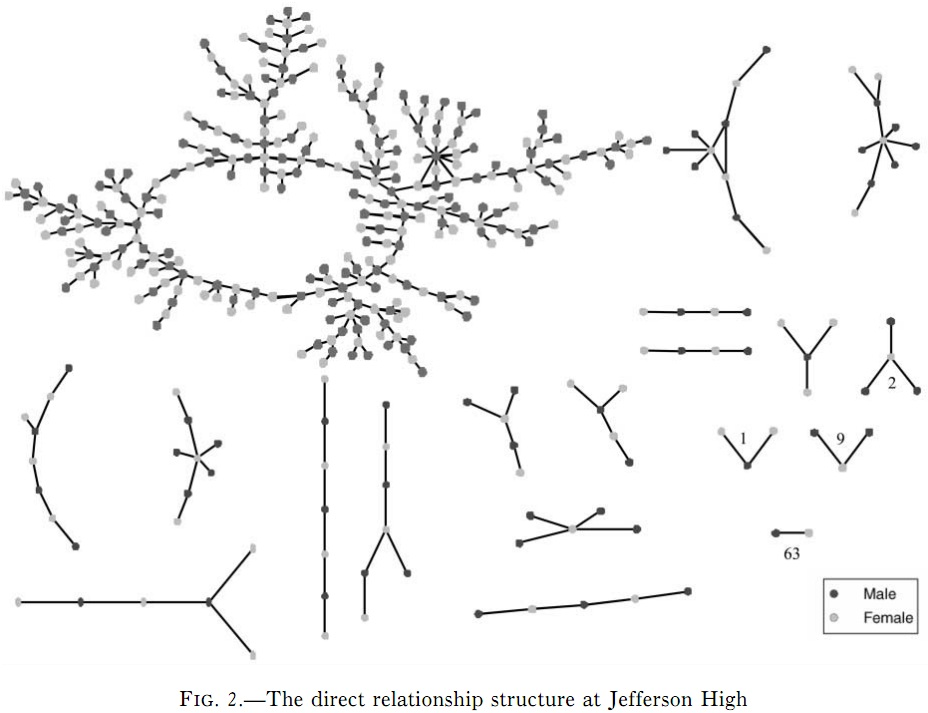
\includegraphics[height=4cm]{images/network.jpg}}\\
				\vspace{0.7cm}
				Sexual ties in high school
			\end{center}
		\end{columns}			
	\end{frame}
	
	\subsection{Data}
	
	\subsubsection{… professional assets}
	
	\begin{frame}[t]{Data stand as \red{professional assets}}
		
\includegraphics[width=\textwidth]{images/oecd.jpg}
	\end{frame}
	
	\subsubsection{… policy expertise}

	\begin{frame}[c]{Data stand as \red{policy expertise}}
		\begin{center}
			\href{http://www.securite-sociale.fr/chiffres/ccss/notesconj/conj200903.pdf}{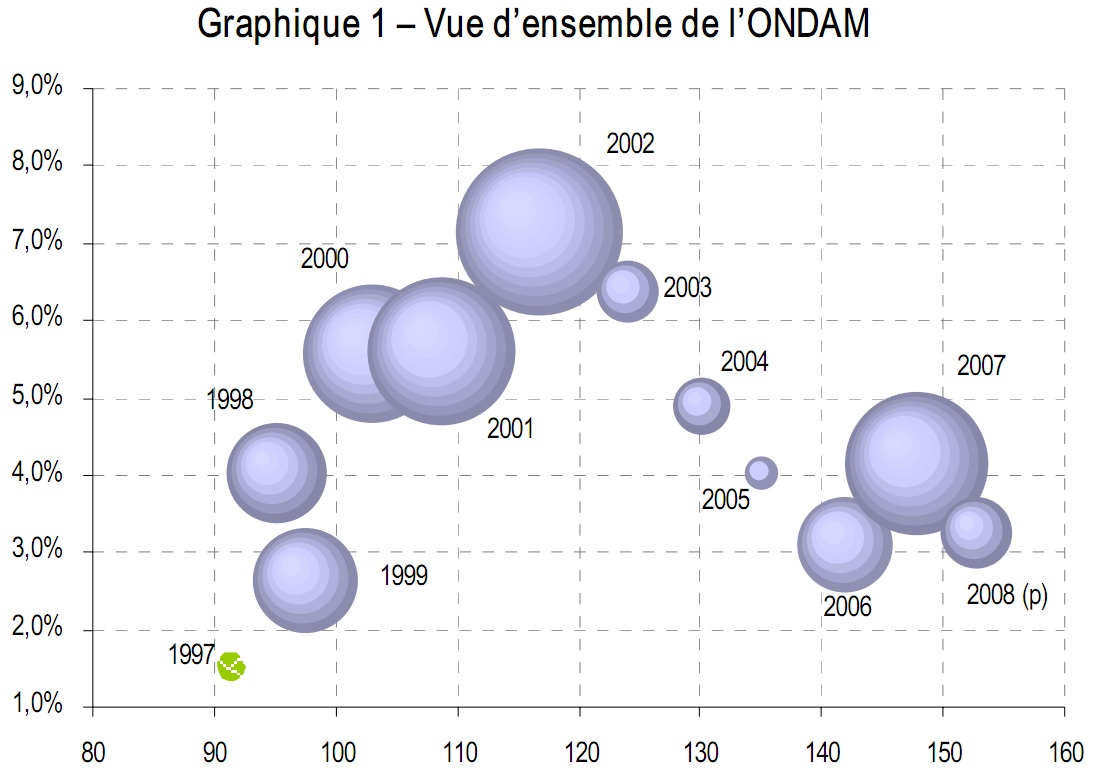
\includegraphics[width=.85\textwidth]{images/ondam.jpg}}
		\end{center}		
	\end{frame}
	
	\subsection{Interpretation}

	\subsubsection{… key to all analysis}
	
	\begin{frame}[c]{\red{Interpretation} is key to all analysis}

		\begin{columns}[T]
			\column{.45\textwidth}
			\begin{center}
				\href{http://jhfowler.ucsd.edu/alone_in_the_crowd.pdf}{\includegraphics[height=4cm]{images/fowler.jpg}}\vspace{1cm}
				Loneliness in social networks
			\end{center}
			\column{.45\textwidth}
			\begin{center}
				\href{http://books.google.fr/books?id=gvgCYyFN7RIC&pg=PA19&lpg=PA19}{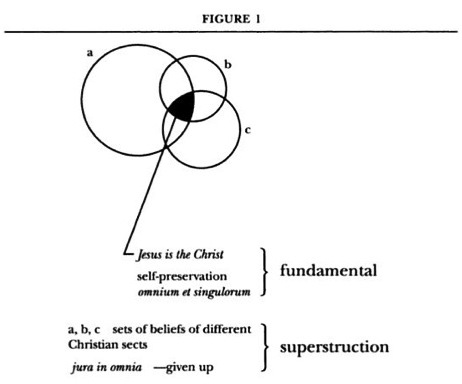
\includegraphics[height=4cm]{images/jesus.jpg}}\vspace{1.05cm}
				Sets of Christian beliefs
			\end{center}
		\end{columns}			
	\end{frame}

	\subsubsection{… difficult}
	
	\begin{frame}[c]{\red{Interpretation} is difficult}

		\begin{columns}[T]
			\column{.45\textwidth}
			\begin{center}
				\href{http://jhfowler.ucsd.edu/alone_in_the_crowd.pdf}{\includegraphics[height=5cm]{images/fowler2.jpg}}\\
				\vspace{0.25cm}
				With explanation
			\end{center}
			\column{.45\textwidth}
			\begin{center}
				
\includegraphics[height=5cm]{images/explain.jpg}\\
				\vspace{0.25cm}
				Without explanation
			\end{center}
		\end{columns}			
	\end{frame}

	\subsubsection{… what this course is about}
	
	\begin{frame}[t]{\red{Interpretation} is what this course is eventually about}
		
		\href{http://www.phdcomics.com/comics.php?f=1219}{\includegraphics[width=\textwidth]{images/productivity.jpg}}
		
		\begin{itemize}
			\item What is the \textbf{measurement} of the axes?
		
			\item What is the \textbf{probability} of 2am being the ``usual'' cutoff point?
		
			\item What is the \textbf{shape} of the time/productivity relationship?
		
		\end{itemize}		
	\end{frame}
	
	\subsection{Biases}
	
	\subsubsection{… internal}
	
	\begin{frame}[t]{Internal biases}

		Statistical reasoning and quantitative methods are services to enhance your interpretation of reality with measurements and probability levels.\vspace{1em}
		
		We will use observational data from social surveys, which have \red{internal limitations}: %\vspace{0.5em}

		\begin{itemize}
			\item Survey design and \textbf{sampling strategy}:\\
			\begin{quote}
			``Please fill in this 367-page long questionnaire''\\
			``Answer our questions and win an iPad! (perhaps)''\\
			``We surveyed knowledge of GLMM among toddlers.''
			\end{quote}
			\item Question design and \textbf{measurement error}:\\
			\begin{quote}			
			``Are you a racial supremacist pig?''\\
			``What do you like most, inflation or \textit{Star Wars}?''\\
			``Do you support Aliina Koospürati’s new coalition?''
			\end{quote}
		\end{itemize}			
			
	\end{frame}
	
	\subsubsection{… external}
	
	\begin{frame}[t]{Further external biases}

		\begin{itemize}
			\item Media coverage
			\item Political spin		
		\end{itemize}	
				
		\href{//}{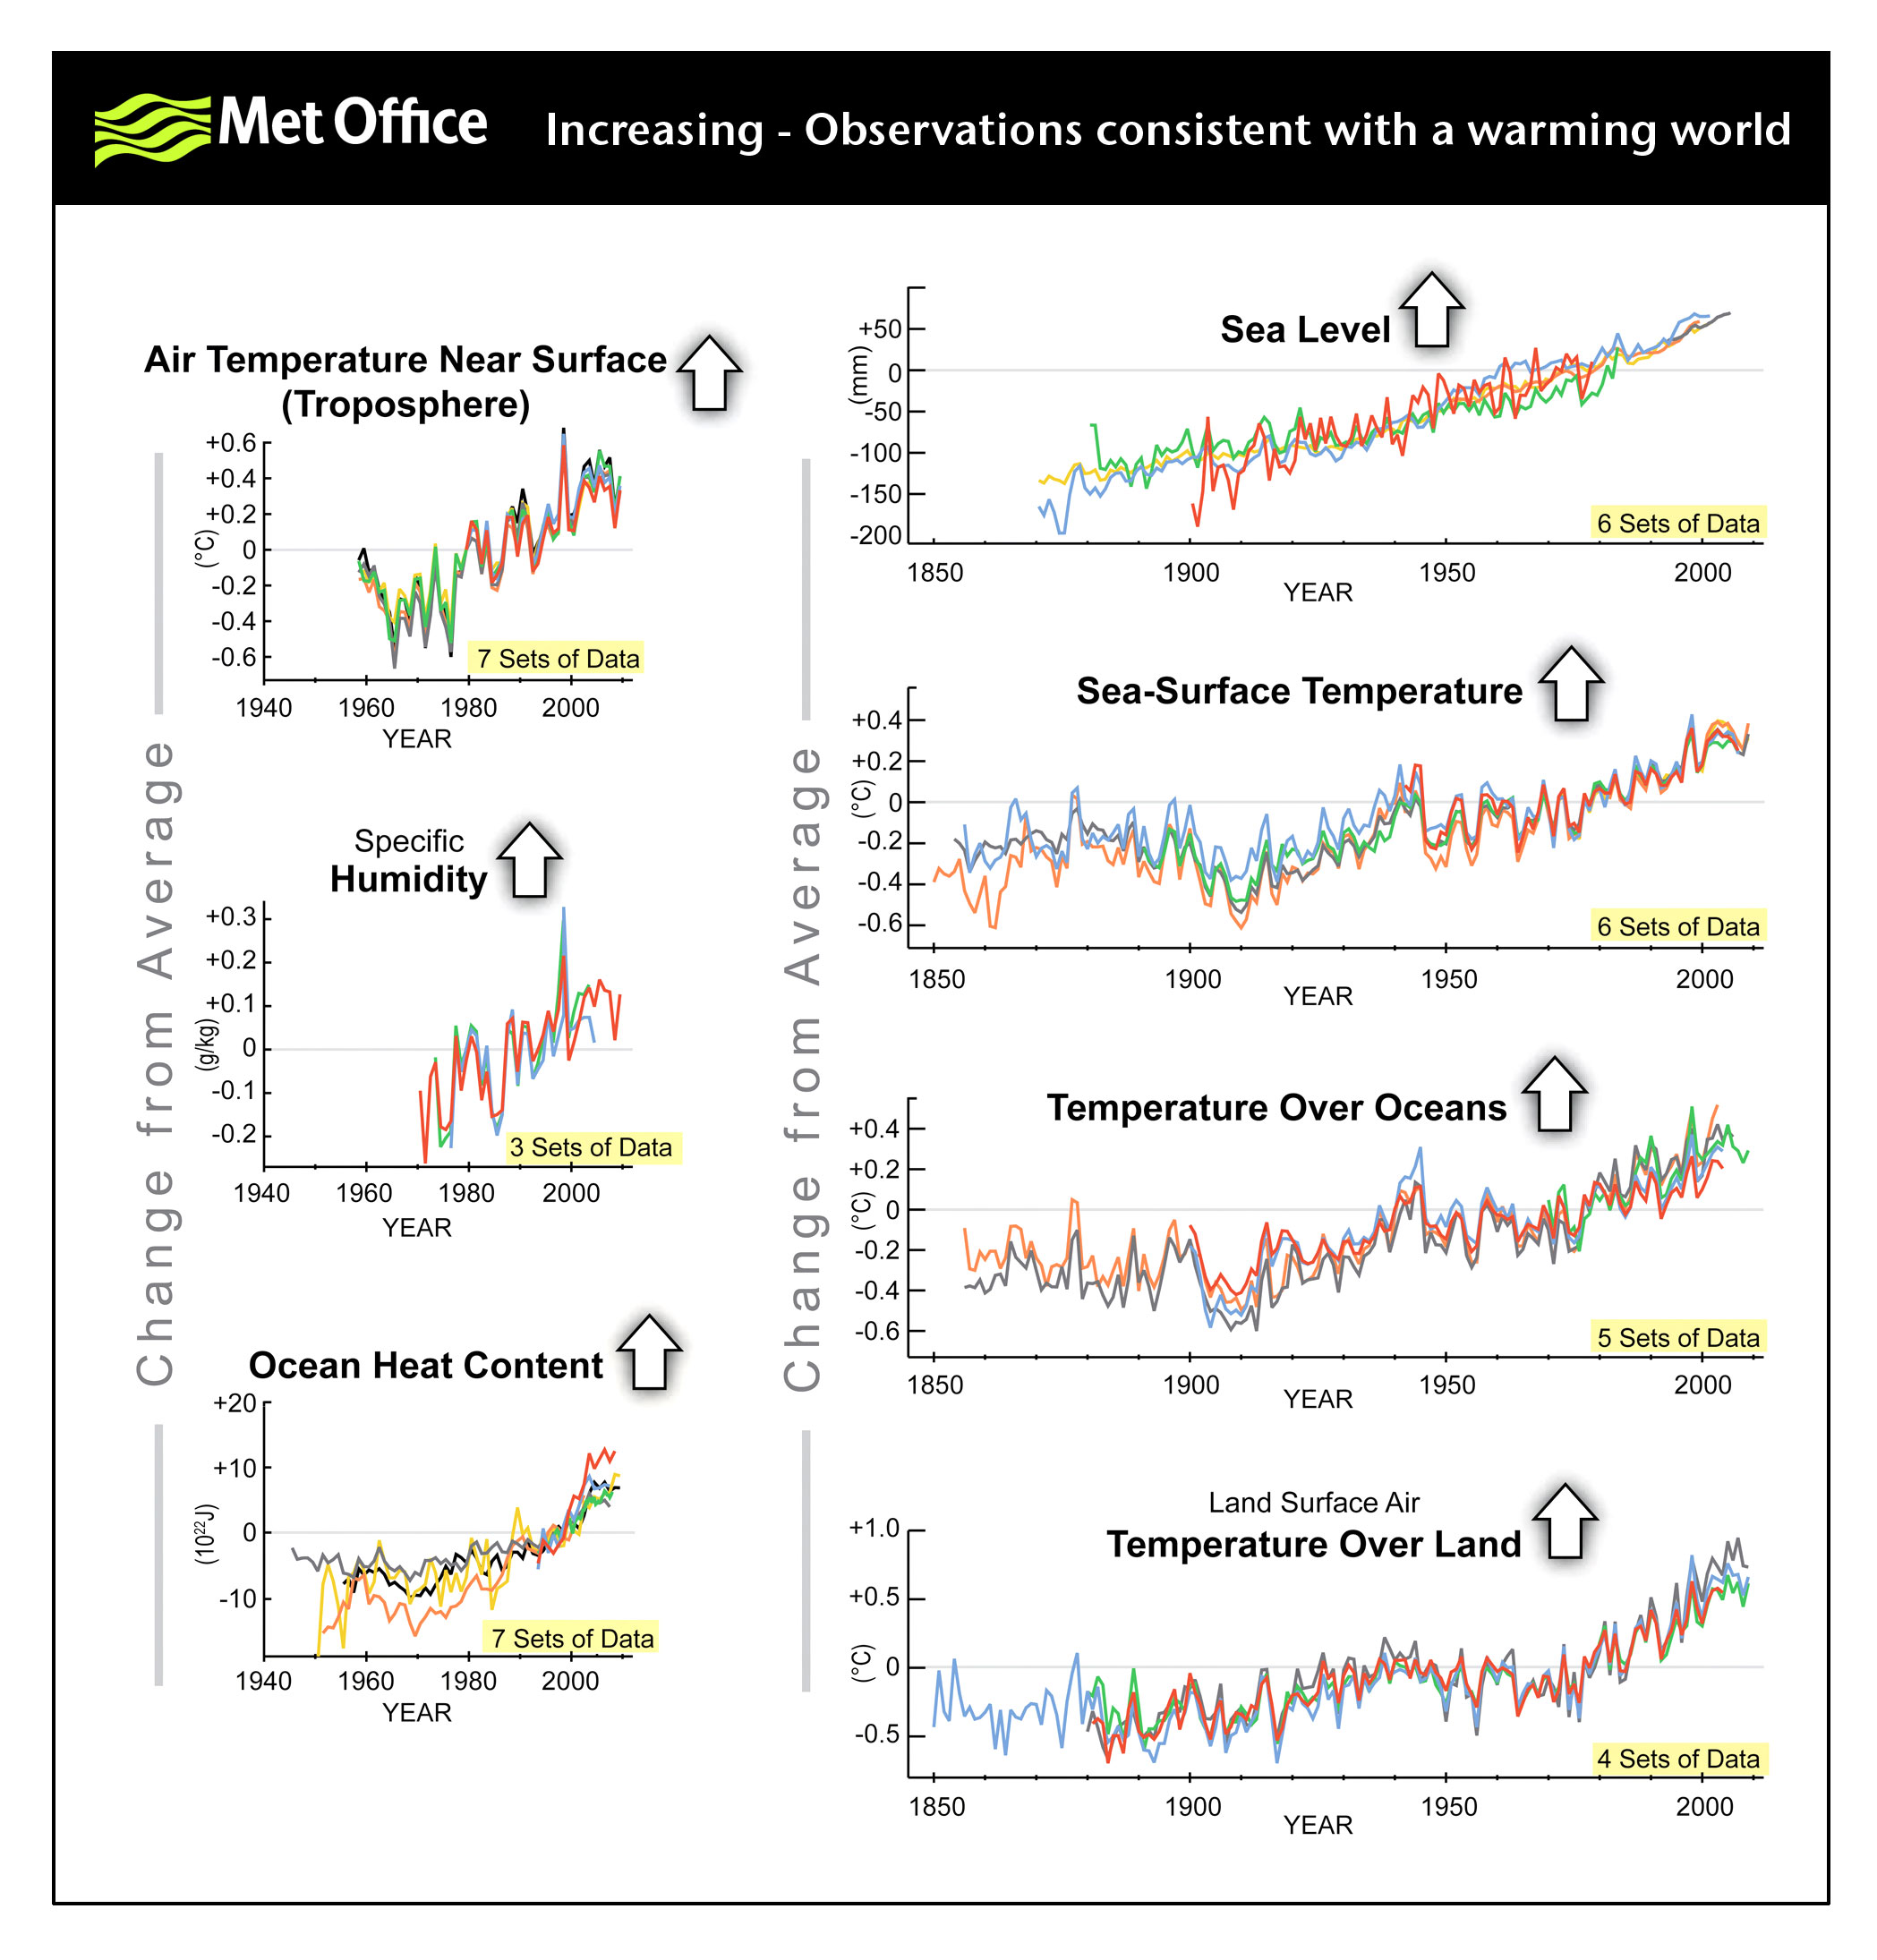
\includegraphics[width=\textwidth]{images/warming.jpg}}
			
	\end{frame}
	
	\subsubsection{… WEIRD}
	
	\begin{frame}[t]{Further WEIRD biases}
		
		\href{http://www2.psych.ubc.ca/~henrich/pdfs/WeirdPeople.pdf}{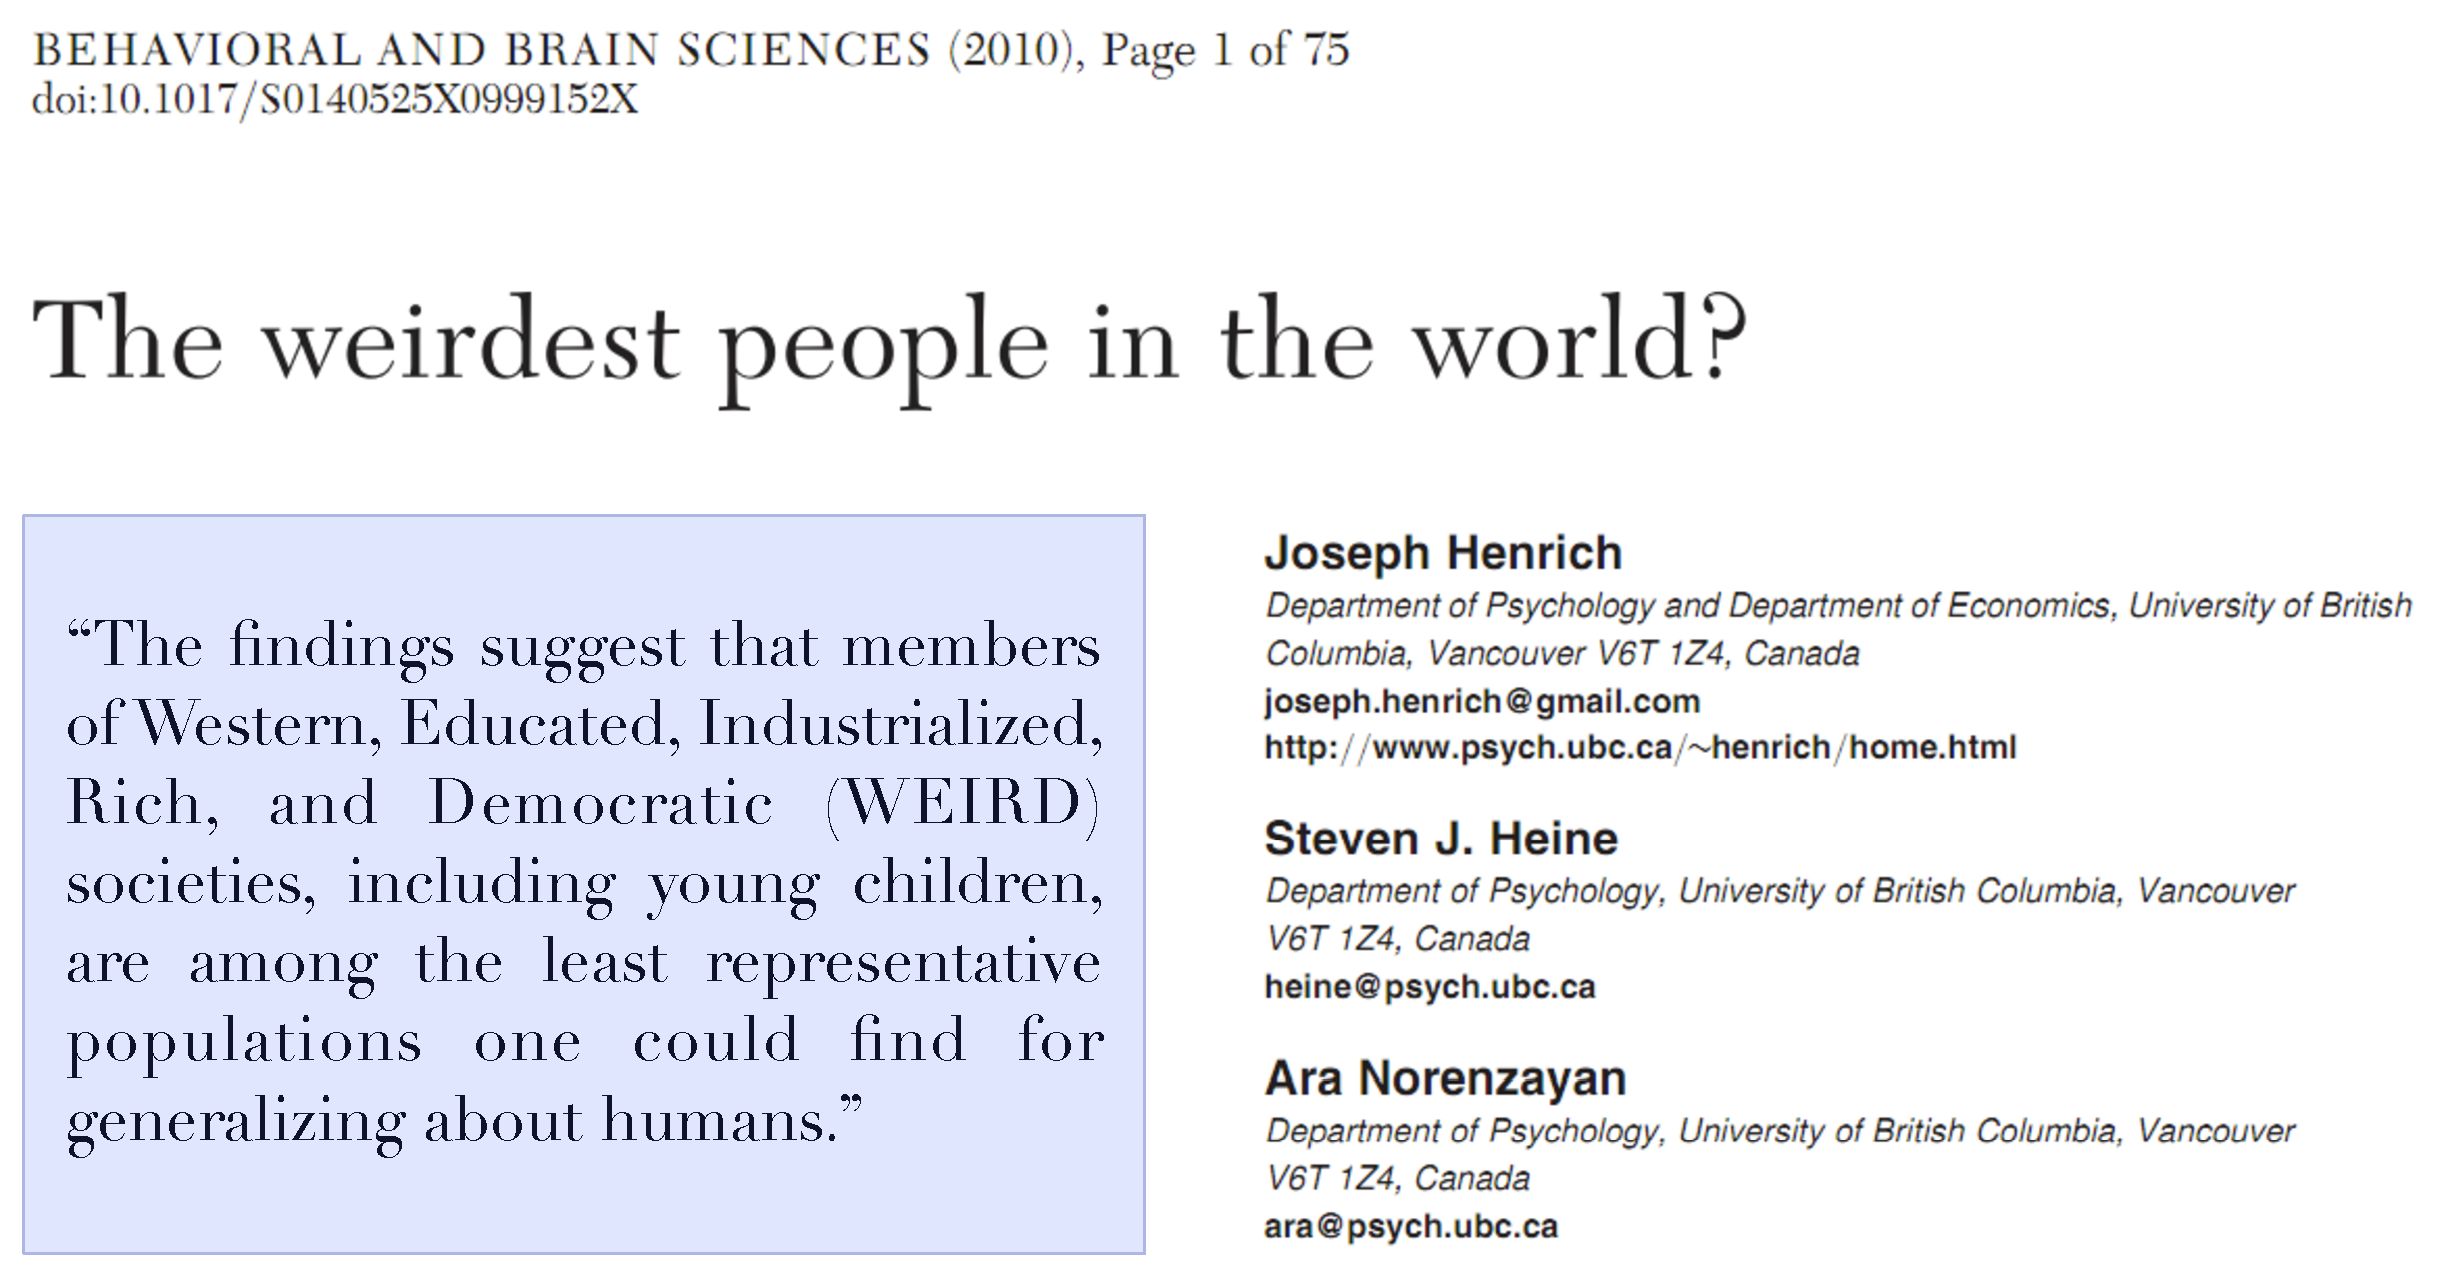
\includegraphics[width=\textwidth]{images/bbs.pdf}}	
	\end{frame}

	\fullslide{images/caravaggio.jpg}
	
	%
	%
	%
	\section{Course}

	\subsection{Objectives}

	\begin{frame}[t]{Learning objectives}

		\begin{itemize}
			\item \textbf{Frequentist statistics}
			\begin{itemize}
				\item Normal distribution
				\item Probability levels
			\end{itemize}
			\item \textbf{Data management}
			\begin{itemize}
				\item Variable transformations
				\item Dataset manipulation
			\end{itemize}
			\item \textbf{Analytical techniques}
			\begin{itemize}
				\item Univariate statistics
				\item Bivariate statistics
				\item Regression modelling
			\end{itemize}
		\end{itemize}	
		
		The course offers an \red{introduction} to ``Statistical Reasoning and Quantitative Methods'' using \red{Stata}. It leaves out much of survey design and nonparametric statistics. It stops before advanced regression modelling and post-frequentist statistics.
	\end{frame}

	\subsection{Requirements}

	\begin{frame}[t]{Requirements}

		\begin{itemize}
			\item \textbf{Homework}
			\begin{itemize}
				\item Handbook readings
				\item Session replication
			\end{itemize}
			Homework deals with \red{statistical theory} and learning \red{Stata programming} for quantitative analysis.
			\item \textbf{Assignments}
			\begin{itemize}
				\item Draft Paper No. 1: data preparation and variable descriptions
				\item Draft Paper No. 2: association
			\end{itemize}
			Assignments deal with the cumulative steps of \red{research design} that are reflected in your final paper.
			\item \red{\textbf{Final paper}}
			\begin{itemize}
				\item Complete do-file
				\item Multiple regression model
				\item Interpretation
			\end{itemize}
		\end{itemize}	
	\end{frame}

	\subsection{Attendance}

	\begin{frame}[t]{Attendance}
		\begin{columns}[T]
			\column[]{.65\textwidth}
			
			Regular attendance is compulsory, but most importantly, \red{homework needs to be done \textbf{on a weekly basis}}, in order to write up Assignments No. 1 and 2.\vspace{1em}
			
			The final paper comes out of this regular coursework and \textbf{cannot}, from experience, be rushed as overnight sessions and other methods to catch up with late work. Sorry.\vspace{1em}

			There is plenty of course material to achieve all requirements and find help, but you will need to \red{read and practice weekly}.
			\column[]{.25\textwidth}
			\begin{center}
			
\includegraphics[width=\textwidth]{images/due-tomorrow.jpg}\vspace{1em}
			
			This won't work.
			\end{center}
		\end{columns}		
	\end{frame}
	
	\subsection{Logistics}

	\begin{frame}[t]{Logistics}
		\begin{columns}[T]
			\column[]{.35\textwidth}
			
			\begin{itemize}
				\item Teaching Pack
				\item Course Website
				\item Student Rep
			\end{itemize}

			No estimation without representation, one (wo)man, one vote, etc.\vspace{1em}
			
			\textbf{Any questions so far?}\vspace{1em}
			Do not worry about \red{deadlines, grades and instruction sets}: these will be discussed in class and sent by email.
			\column[]{.55\textwidth}
			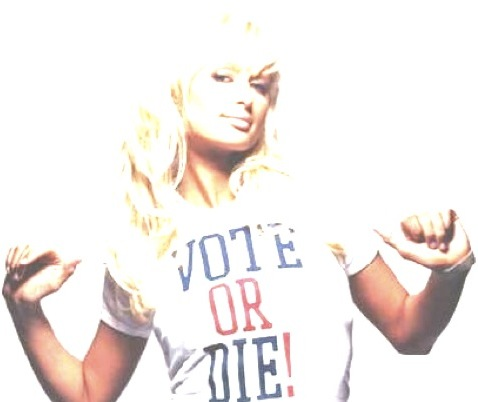
\includegraphics[height=.8\textheight]{images/vote.jpg}
		\end{columns}		
	\end{frame}
	
	%
	% Break here.
	%
	
	\section{Computers}

	\begin{frame}[t]{Computers}
	
		\begin{columns}[T]
			\column{.4\textwidth}
			
			\begin{itemize}
				\item Music players
				\item Facebook terminals
				\item Porn stashes
			\end{itemize}

			Despite the appearances, computers are not just that.\vspace{1em}			
			They can also be used to \red{do}, like, serious stuff.
			\column{.4\textwidth}
			
\includegraphics[width=\textwidth]{images/dilbert-porn.jpg}
		\end{columns}
	
	\end{frame}		

	\subsection{Computer skills}

	\begin{frame}[t]{Computer skills}
		\begin{itemize}
			\item \textbf{Section 2 of the Stata Guide} will walk you through the most essential notions that you must be confident with:
			
			\begin{itemize}
				\item Files (size, names, extensions, compression)
				\item System (memory, folders/directories, file/folder paths)
				\item Code (programming, replication, debugging)
			\end{itemize}
			
			\item \textbf{Using your personal computer} is preferrable due to limitations in administrator privileges with university computer lab machines.
			
			\item \textbf{Backup your files every week} on at least two different locations. Using a USB key or a Gmail account will do.

		\end{itemize}

		Personal pledge:
		\begin{quote}
		I hereby declare that, if no single case of data loss is reported throughout the semester, I will buy a drink to the whole class.		
		\end{quote}

	\end{frame}

	\subsubsection{Example: Saving files}
	
	\begin{frame}[t]{Example: Saving files}

		\textbf{Do not save online files by single-clicking them}. This is good for opening holiday pictures attached to an email on the fly, not for working with files that often need to be decompressed and archived.\vspace{1em}
		
		Instead, use the \red{``	Save As…''} or \red{``Download As…''} right-click menu item of your browser to save the file at a precise location.\vspace{1em}
		
		\includegraphics[width=\textwidth]{images/save.jpg}	
	\end{frame}
	
	\begin{frame}[t]{Computer skills}
		It would be best for all to start the course with computer issues solved. Let's pause here and solve as many issues right now.\vspace{1em}
	
		\includegraphics[width=\textwidth]{images/dilbert-complit.jpg}

	\end{frame}

	\begin{frame}[t]{Computer skills}
		Everything you will learn in this course will serve with other projects.\vspace{1em}
	
		\href{http://f.briatte.org/research/kmaps/}{\includegraphics[width=\textwidth]{images/kmaps.jpg}}

	\end{frame}

	\subsection{First Stata run}

	\begin{frame}[t]{First Stata run}
	
	Open Stata and type the following commands, shown \code{in blue}, in the \textbf{$\square$ Command} window:
	
	\begin{itemize}
		\item \code{set mem 500m} will show changes in \textbf{$\square$ Results} and \textbf{$\square$ Review}.
			
			(ignore this command if you are running Stata 12+)
				
		\item \code{sysuse lifeexp} loads data and variables in \textbf{$\square$ Variables}.
				
		\item \code{edit} opens the \textbf{$\square$ Data Editor}  with the \code{lifeexp.dta} dataset.

		Close the Data window.
		
		\item \code{scatter lexp safewater} creates your first \textbf{Stata graph}!
		
		Close the Graph window.
		
		\item \code{doedit} opens an empty, untitled \red{do-file} in the \textbf{$\square$ Do-file Editor}.
	\end{itemize}
	
	\end{frame}
	
	\begin{frame}[t]{First Stata run}
	
	\begin{itemize}
		\item Write the following lines in your do-file:
		
		\code{* First do-file.}
		
		\code{sysuse lifeexp, clear}
				
		\code{scatter lexp safewater}
		
		\code{clear}
		
		\item Select the four lines of your do-file and use the \textbf{Tools $\triangleright$ Execute Selection (do)} menu to run them. To finish, save up your work:
		
		\begin{itemize}
			\item Save the Graph with \textbf{File $\triangleright$ Save}, using the \code{.jpg} format.
			\item Save the do-file, also with \textbf{File $\triangleright$ Save}, using the \code{.do} format.
		\end{itemize}
		
		The do-file allows to \red{replicate} your results. Using that do-file, you can share your results on life expectancy and access to clean water with any other Stata user.
	\end{itemize} 
			
	\end{frame}
	
	\section{Stata}

	\subsection{Stata application}

	\begin{frame}[t]{Stata \red{application}}
		\begin{columns}[T]
			\column{.7\textwidth}
			\begin{itemize}
				\item \textbf{Recent PC/Macs can run Stata 10/12.}\\ Make sure that you have a reasonable amount of memory and disk space available.
				
				\item \textbf{``SE'' stands for `Special Edition.'}\\ Other editions of Stata come with slightly different software characteristics.
				
				\item \textbf{Additional packages are downloadable.}\\ The main online source is the  Statistical Software Components (SSC) server.

			\end{itemize}
			
			Software details:
			
			\url{http://www.stata.com/}

			\column{.3\textwidth}
			\includegraphics[width=.25\paperwidth]{images/icon-stata11.jpg}
		\end{columns}
	\end{frame}

	\subsubsection{Operationalization}

	\begin{frame}[t]{Operationalization}
									
		\comm{Allocate 500MB memory (use in Stata 11-).}
					
		\code{set mem 500m, perm}

		\comm{Suppress screen breaks permanently.}

		\code{set more off, perm}

		\comm{Install the `fre' package.}

		\code{ssc install fre}
						
		\begin{itemize}
			\item Lines starting with \texttt{*} are \textbf{comments}, others are \textbf{commands}. Syntax colouring (supported by Stata 11+) differentiates them.
			\item The \code{perma} option requires \textbf{system administrator privileges}. Without the options, the commands have to be run at each launch.
			\item Installing packages also requires administrator system privileges and \textbf{Internet access} to reach the SSC server.			
		\end{itemize}
	\end{frame}

	\subsection{Stata datasets}

	\begin{frame}[t]{Stata \red{datasets}}
		\begin{columns}[T]
			\column{.6\textwidth}
			\begin{itemize}
				\item A Stata dataset is a specific file format of quantitative data that ends with the \code{.dta} file extension.
				
				\item Stata opens datasets from the \textbf{File $\triangleright$ Open} menu or with the \code{use} command, often with the \code{clear} option.
				
				\item Other formats are supported through import commands, e.g. \code{insheet} for [comma-separated values] CSV files.
			\end{itemize}
						
			Examples:
			
			\begin{itemize}
				\item \textbf{Datasets} in the \code{SRQM} folder

				\item \textbf{Course Website}		
			\end{itemize}
			
			\column{.3\textwidth}
			
\includegraphics[width=.25\paperwidth]{images/icon-dta.jpg}
		\end{columns}
	\end{frame}
	
	%
	%
	% commands to browse data: cd, use , edit
	%
	%
	\subsubsection{Operationalization}

	\begin{frame}[t]{Operationalization}
	
		Load the National Health Interview Survey (2009):
		
		\begin{itemize}
		
			\item Using the \textbf{File $\triangleright$ Open} menu:
			
			\begin{itemize}
				\item Select ``\textbf{Stata dataset (.dta)}'' in the file extension menu.
				\item Open \textbf{Teaching Pack $\triangleright$ Datasets $\triangleright$ \red{nhis2009.dta}}.
			\end{itemize}	
			
			\item Using the Stata command line:
			
			\comm{Set the path to your Teaching Pack folder.}
			
			\code{cd "/Users/fr/Documents/SRQM/"}
			
			\comm{Load the dataset by calling its file name.}
			
			\code{use "Datasets/nhis2009.dta"}
			
		\end{itemize}
		
		\red{Note}: the working directory setting called by the \code{cd} command is system-dependent and must reflect your own folder hierarchy.
	
	\end{frame}		
	
	\subsection{Stata do-files}

	\begin{frame}[t]{Stata \red{do-files}}
		\begin{columns}[T]
			\column{.6\textwidth}
			\begin{itemize}
				\item A do-file is a plain text file holding a list of Stata commands, that can be edited from any \textbf{plain text editor}.
				
				\item Stata opens and edits do-files from the \textbf{File $\triangleright$ Open} menu or through the \code{doedit} command.
				
				\item The \code{do} and \code{run} commands will try to execute a full do-file in order to replicate its results.
				
			\end{itemize}
						
			Examples:
			
			\begin{itemize}
				\item \textbf{Teaching Pack $\triangleright$ Replication}

				\item \textbf{Course Website}		
			\end{itemize}

			\column{.3\textwidth}
			\includegraphics[width=.25\paperwidth]{images/icon-do.jpg}
		\end{columns}
	\end{frame}

	%
	%
	% example with comments; explain sequential order
	%
	%		
	
	\subsubsection{Operationalization}
	
	\begin{frame}[t]{Operationalization}
	
		\begin{itemize}
			\item Using the \textbf{File $\triangleright$ Open} menu:
			
			\begin{itemize}
				\item Select ``\textbf{Stata do-file (.do)}'' in the file extension menu.
				\item Open \textbf{Teaching Pack $\triangleright$ Replication $\triangleright$ \red{week1.do}}.
			\end{itemize}			
			
			\item Locate the following commands:

			\code{d year sex weight raceb // describe a few variables}
						
			\code{keep if year==2009 // keep observations for year 2009}
						
			\item Select both command lines and run (execute) them together:
			
			\begin{itemize}
				\item You can select \comm{commented} lines when running a command, as they have no effect on how Stata executes the rest of the code.
				\item Type \textbf{Ctrl-D} (PC) or \textbf{Cmmd-Shift-D} (Mac) to run the selected command(s) from the keyboard.
				
			\end{itemize}
\item Alternately, use the \textbf{``Execute (do)'' icon} from the do-file toolbar:
				
\includegraphics[width=.9\textwidth]{images/scrn-do.jpg}
		\end{itemize}	
	
	\end{frame}				

	\subsection{Other components}

	\begin{frame}[t]{Other components}
			
		\begin{itemize}
		
			\item \textbf{Log files} are plain text files that hold commands and their results, used for replication purposes.
			
			\begin{itemize}
				\item Stata has its own \code{SMCL} format but we will prefer plain text \code{.log} files.
				\item Log files are optional but recommended to keep track of your work.
			\end{itemize}	
			
			\item \textbf{Graphs} are picture files that you produce through specific Stata commands, for visualization purposes.
			
			\begin{itemize}
				\item Stata has its own \code{GPH} format but we will prefer saving as \code{.jpg}.
				\item Use the \code{name()} option to store a graph and leave its window open, and then use the \code{graph export} command to save it on disk.
				\item Alternately, save a graph manually with the \textbf{File $\triangleright$ Save} menu, or with the \textbf{``Save'' icon} from the graph toolbar.
				
\includegraphics[width=.9\textwidth]{images/scrn-savegraph.jpg}
			\end{itemize}	
					
		\end{itemize}
			
	\end{frame}	

	\subsubsection{Operationalization}
	
	\begin{frame}[t]{Operationalization}
	
		Return to Stata and to the \textbf{\red{week1.do}} file.
		
		\begin{itemize}
			\item To log your work, type:
			
			\code{log using week1.log, replace}
			
			\begin{itemize}
				\item When opening a log, remember to use the \code{.log} extension.
				\item The log file will be saved in your working directory. The \code{replace} option overwrites any previously log file at that location.
				\item Stata automatically stops logging when you quit it. The \code{log close} and \code{exit} commands respectively perform the same operations.
			\end{itemize}
			
			\item To plot a variable as a histogram, type:
			
			\code{histogram weight, bin(20) name(weight, replace)}
			
			\begin{itemize}
				\item When saving the graph, remember to select the \textbf{JPG} format.
				\item The \code{replace} option is required to overwrite any previous graph with that name. Use it systematically to avoid errors.
				\item This graph uses the \code{bin} and {name} options, and might require further options to produce an appropriate visualization of the variable.
			\end{itemize}
		\end{itemize}	
	
	\end{frame}		

	\section{Help}

	\begin{frame}[t]{Getting help}
		Quantitative methods systematically require extensive documentation. Locating help resources is a course requirement and a skill in itself. When asked for help, we will frequently refer to these resources:

		\begin{itemize}
			\item \textbf{Course material}:

			\begin{itemize}
				\item Stata Guide
				\item Course slides and emails
				\item Handbook chapters
			\end{itemize}			
			
			\red{Start reading the \textbf{\href{http://f.briatte.org/teaching/quanti/}{Stata Guide}.}}
			
			\item \textbf{Other material}:
			
			\begin{itemize}
				\item Stata \code{help} pages
				\item Stata tutorials
			\end{itemize}
			
			\red{Start exploring the \textbf{\href{http://f.briatte.org/teaching/quanti/}{Course Website}.}}
		\end{itemize}

	\end{frame}

	\subsection{Stata Guide}

	\begin{frame}[t]{Stata Guide}
		\begin{columns}[T]
			\column{.5\textwidth}
			\textbf{The Stata Guide} is a course handbook which we co-write with Ivaylo. Its chapters cover virtually all course sessions.\vspace{1em}
			
			\textbf{The Guide is work in progress}: please email comments, questions and corrections, and watch for updates during the course.
			
			\column{.5\textwidth}
			\includegraphics[width=.45\paperwidth]{images/stata-guide.jpg}
		\end{columns}
	\end{frame}
				
	\subsection{Course slides}

	\begin{frame}[t]{Course slides}

		The course slides contain very basic guidance and are \red{absolutely insufficient} to complete the course requirements.\vspace{1em}
		
		More generally, slideware is a teaching aid, \red{not a learning tool}. Watching slides does not compensate documentation.\vspace{1em}
	
		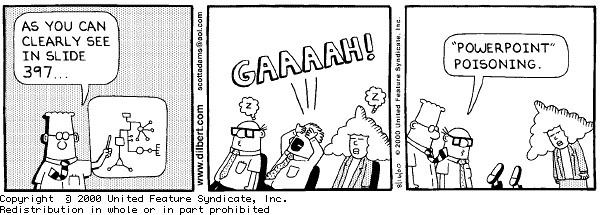
\includegraphics[width=\textwidth]{images/dilbert-ppt.jpg}

	\end{frame}

	\subsection{Course slides}

	\begin{frame}[t]{Course emails}

		The course emails will be our lifeline, with insanely detailed \red{instructions about your homework}, and more. Read them carefully.\vspace{1em}
		
		We will also answer all emails about the course as quickly as possible. \textbf{\red{Include both instructors on emails.}}\vspace{1em}
		
		Do not forget to email with a subject that starts with \textbf{``SRQM:''} to help us parse our mailboxes, as in ``SRQM: Question on recoding.''\vspace{1em}
		
		Possible email subjects:
		
		\begin{quote}
		``SRQM: Issue with plotting sex, drugs and rock'n'roll''
		
		``SRQM: Assignment No. 2, Briatte and Petev''
		
		``SRQM: Where has the cherry blossom of our youth gone?''
		
		``SRQM: Why are scatterplots with ordinal data so ugly?''
		\end{quote}
	
	\end{frame}

	\subsection{Handbook chapters}

	\begin{frame}[t]{Handbook chapters}

		\begin{quote}
		``The fact that they looked it up in a book just shows that they don't get the idea of truthiness at all... You don't look up truthiness in a book, you look it up in your gut.''\\(Stephen Colbert to the Associated Press)
		\end{quote}\vspace{1em}
		
		\begin{itemize}
			\item \textbf{Understanding the statistical theory} that underlies the rest of your practical tasks will inevitably show up in your analysis.
			\item \textbf{Truthiness will just not work with us}. It might with a sloppy newspaper or polling institute, but not with academics.
			\item \textbf{Aim at understanding the theory once}, which is enough at the introductory level. Once is enough, but once, no less.
		\end{itemize}

	\end{frame}

	\subsection{Stata help pages}

	\begin{frame}[t]{Stata \code{help} pages}

		Type \code{help su} and skim-read the page:

		\begin{itemize}
			\item \textbf{Syntax indications} help correcting a great deal of coding errors.
			\item \textbf{Options lists} help improving your code, and especially graphs.
			\item \textbf{Examples} illustrate how the commands can be used effectively.
		\end{itemize}
		
		Remarks on Stata command syntax:
		
		\begin{itemize}
			\item \code{su} is the abbreviated version of the \code{summarize} command. Command shorthands are underlined in the Stata help pages.
		
		You can abbreviate tons of Stata commands and options: \code{h li}, for example, opens the \code{help} page for the \code{list} command.
		
			\item Variable names cannot be abbreviated, but you can refer to groups of variables: \code{su v1-v5} is equivalent to \code{su v1 v2 v3 v4 v5}, and \code{su var*} will treat all variables named \code{var1 var2 var3} etc.
		\end{itemize}

	\end{frame}

	\subsection{Stata tutorials}

	\begin{frame}[t]{Stata \red{tutorials}}

		Reading documentation goes hand in hand with \red{lots of practice}:

		\begin{itemize}
			\item \textbf{Replicate all course sessions} to get familiar with the commands introduced during class.
			\item \textbf{Read the Stata Guide} and work through the examples, while working on your own data and project.
			\item \textbf{Find online tutorials} on the specific aspects that you find most problematic, such as recoding.
		\end{itemize}
		
		Links to the most useful resources:
		
		\url{http://f.briatte.org/teaching/quanti/\#stata}
		
		\vspace{1em}
		
		Examples of excellent online tutorials:
		
		\url{http://www.princeton.edu/wwac/academic-review/stata/}
				
		\url{http://www.ats.ucla.edu/stat/stata/default.htm}
	\end{frame}

	\section*{Welcome}

	\begin{frame}[t,plain]
			\vspace{.2\paperwidth}
		\begin{center}
			{\Large \red{Welcome}, and thank you.}\\
			\vspace{.1\paperwidth}
			\href{http://xkcd.com/552/}{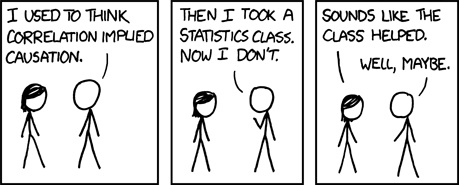
\includegraphics[height=4cm]{images/xkcd-correlation.jpg}}
		\end{center}
	\end{frame}

\end{document}

